\documentclass[11pt]{article}
\usepackage{amsmath,amstext,amsfonts,amssymb,amsthm,epsfig,epstopdf,url,array}
\usepackage[margin=1in]{geometry}
\usepackage{xcolor}
\usepackage{graphicx}
\usepackage{times}
\usepackage{authblk}

\theoremstyle{plain}
\newtheorem{thm}{Theorem}[section]
\newtheorem{lem}[thm]{Lemma}
\newtheorem{prop}[thm]{Proposition}
\newtheorem{cor}[thm]{Corollary}
\newtheorem{defn}[thm]{Definition}
\newtheorem{claim}[thm]{Claim}

\theoremstyle{definition}
\newtheorem{con}{Conjecture}[section]
\newtheorem{exa}{Example}[section]
\newtheorem*{sol}{Solution}
\newtheorem{cdef}{Definition}[section]


\theoremstyle{remark}
\newtheorem{rem}{\textbf{Remark}}
\newtheorem*{note}{\color{blue}\textbf{Note}}
\usepackage{qtree}


\usepackage{hyperref}

\usepackage[nameinlink,noabbrev,capitalize]{cleveref} 
\crefalias{subequation}{equation}
\crefalias{thm}{theorem}


% to make cleveref print ``Lemma'' for lemma
\let\oldlemma\lem
\renewcommand{\lem}{%
  \crefalias{thm}{lem}% Theorem counter now looks like Lemma
  \oldlemma}
\Crefname{lem}{Lemma}{Lemmas}

% to make cleveref print ``Definition for definition
\let\olddefn\defn
\renewcommand{\defn}{%
  \crefalias{thm}{defn}% Theorem counter now looks like Definition
  \olddefn}
\Crefname{defn}{Definition}{Definitions}

% to make cleveref print ``Remark for remark
\let\oldrem\rem
\renewcommand{\rem}{%
  \crefalias{thm}{rem}% Theorem counter now looks like Remark
  \oldrem}
\Crefname{rem}{Remark}{Remarks}

% to make cleveref print ``Corollary for corollary
\let\oldcor\cor
\renewcommand{\cor}{%
  \crefalias{thm}{cor}% Theorem counter now looks like Corollary
  \oldcor}
\Crefname{cor}{Corollary}{Corollaries}

% to make cleveref print ``Claim for claim
\let\oldclaim\claim
\renewcommand{\claim}{%
  \crefalias{thm}{claim}% Theorem counter now looks like Claim
  \oldclaim}
\Crefname{claim}{Claim}{Claims}

% to make cleveref print ``Proposition for prop
\let\oldprop\prop
\renewcommand{\prop}{%
  \crefalias{thm}{prop}% Theorem counter now looks like Prop
  \oldprop}
\Crefname{prop}{Proposition}{Propositions}

% to make cleveref print ``Conjecture for conj
\let\oldcon\con
\renewcommand{\con}{%
  \crefalias{thm}{con}% Theorem counter now looks like Con
  \oldcon}
\Crefname{con}{Conjecture}{Conjectures}

% Editing commands requiring color package
\newcommand{\add}[1]{\textcolor{blue}{#1}}
\newcommand{\delete}[1]{\textcolor{red}{#1}}
\definecolor{darkgrn}{rgb}{0, 0.8, 0}
\newcommand{\modified}[1]{\textcolor{darkgrn}{#1}}
\definecolor{maroon}{rgb}{0.85, 0.0, 0.1}
\newcommand{\todo}[1]{\textcolor{maroon}{#1}}

\newcommand{\txbl}[1]{\textcolor{blue}{#1}}
\newcommand{\txrd}[1]{\textcolor{red}{#1}}
\newcommand{\txgr}[1]{\textcolor{green}{#1}}
\newcommand{\txcr}[1]{\textcolor{crimson}{#1}}


% shortcut commands
\newcommand{\sym}[1]{\mathcal{S}^{#1}}

\title{Robust Feasibility of Systems of Quadratic Equations Using Topological Degree Theory}

%\author{Krishnamurthy Dvijotham\thanks{\affil{Google DeepMind}}
%    \hspace*{0.3in}
%  Bala~Krishnamoorthy\thanks{\affil{Washington State University}}
%  \hspace*{0.3in}
%  Benjamin Rapone\footnotemark[2]
%}

\author[*]{Krishnamurthy Dvijotham}
\author[**]{Bala~Krishnamoorthy}
\author[**]{Benjamin Rapone}
\affil[*]{Google DeepMind}
\affil[**]{Wahington State University}

\usepackage{csquotes}


\begin{document}

\maketitle

\begin{abstract}
  We consider the problem of measuring the \emph{margin of robust feasibility} of solutions to a system of nonlinear equations.
%  \txgr{Define robustness margin informally here... }\\
  This problem turns out to be NP-hard in general.
  We study the special case of a system of quadratic equations, which shows up in many practical applications such as the power grid and other infrastructure networks. 
  We develop approaches based on topological degree theory to estimate bounds on the robustness margin of such systems.
  Our methods use tools from convex analysis and optimization theory to cast the problems of checking the conditions for robust feasibility as a nonlinear optimization problem.
  We then develop \emph{inner bound} and \emph{outer bound} formulations for this optimization problem, which could be solved efficiently to derive lower and upper bounds, respectively, for the margin of robust feasibility.
  We evaluate our approach numerically on standard instances taken from the MATPOWER database of AC power flow equations that describe the steady state of the power grid.
  The results demonstrate that our approach can produce tight lower and upper bounds on the radius of robust feasibility for such instances.
\end{abstract}


\section{Introduction} \label{sec:intro}  
\section{Introduction} \label{sec:intro}  

Solving systems of equations is ubiquitous in computational mathematics.
In many applications, these problems are made challenging due to the functions in the equations being nonlinear and/or nonconvex.
Another aspect adding to the problem complexity is the uncertainty in the problem parameters.
Our work is motivated by two central computations performed as part of power systems operations are power flow (PF) studies and optimal power flow (OPF).
PF studies ensure the power grid state (i.e., voltages and flows across the network) will remain within acceptable limits in spite of contingencies (e.g., loss of a generator or transmission line) and other uncertainties (e.g., shifting demand or renewable sources of power).
OPF seeks further to choose values for controllable assets in the system (e.g., generators whose rate of power production could be controlled) so as to meet demand at minimum cost.
These problems have inherent nonlinearities and nonconvexities, making them hard to solve in their natural form.
  
To further complicate the problem, the rapid adoption of renewable energy sources such as wind and solar energy is adding unprecedented uncertainties to modern power systems.
Since these sources depend on the weather, their energy output is not perfectly controllable.
In fact, this output can be forecasted with only limited accuracy.
While demand-side flexibility can be used to balance fluctuations in solar and wind generation, its amount can in turn be difficult to predict \cite{mathieu2011examining,taylor2015uncertainty}.
Due to all these uncertainties, it is increasingly difficult to ensure there is sufficient power generation to meet demand while accounting for losses and network limits.

\medskip
We study quadratic systems of equations with parameters, and take a \emph{robust viewpoint} of uncertainty.
Specifically, we aim to quantify the worst-case impact of uncertainty in parameters on feasibility.
To this end, We study the \emph{robust feasibility problem}, which includes the robust version of the standard PF problem as a special case.
The power system can be described by a system of nonlinear equations in a set of variables that capture the state of the power grid, i.e., voltages at every point in the power network, and include the controllable inputs as well as uncertain inputs.
In the main PF problem, we are given a fixed value of the controllable inputs and an uncertainty set for the uncertain inputs.
The goal of the robust feasibility problem is to characterize whether the system has a solution within specified bounds (capturing engineering limits on voltages, flows, etc.) for {\em each} choice of the uncertain inputs in the uncertainty set.

\medskip
More concretely, we study a system of quadratic equations $F(\vx)=\vu$ where $F: \R^n \mapsto \R^n$ is quadratic in $\vx$ for $\vx,\vu \in \R^n$.
  We consider situations where the parameters $\vu$ are uncertain, and we are interested in guaranteeing the existence of a solution to $F(\vx) = \vu$ within limits on $\vx$ and $\vu$.
We draw on results from topological degree theory and Borsuk's theorem from algebraic topology and nonlinear analysis to develop tests for existence of solutions.
Using ideas from optimization such as convex relaxations of quadratic constraints, we develop rigorous and efficient algorithms based on these tests for robust feasibility.
We develop efficient implementations of these algorithms capable of scalably solving large instances of PF problems.
While we use power systems as the main application area, the methods we develop are fairly general, and could be applied to problems in other domains as well, e.g., stochastic processes and gas distribution networks.

\subsection{Our Contributions}
  We study systems of quadratic equations, and define a \emph{robustness margin} as a measure of the system's robust feasibility (see \cref{RobustDef}).
  We develop approaches based on topological degree theory to estimate bounds on the robustness margin of such systems (see \cref{sec:theory}).
  We use tools from convex analysis and optimization theory to cast the problems of checking the conditions for robust feasibility as a nonlinear optimization problem.
  We then develop \emph{inner bound} (\cref{sec:inbdform}) and \emph{outer bound} (\cref{sec:outbdform}) formulations for this optimization problem, which could be solved efficiently to derive lower and upper bounds, respectively, for the margin of robust feasibility.
  We evaluate our approach numerically on standard instances taken from the MatPower database of AC power flow equations that describe the steady state of the power grid (\cref{sec:numstd}).
  The results demonstrate that our approach can produce tight lower and upper bounds on the robustness margin for such instances.

\subsection{Related Work}

Robust feasibility and optimization have been well-studied by both the optimization and topology communities. 
What is lacking is an approach that can guarantee and quantify robust feasibility on large scale systems in an efficient manner. 
In this article we address this deficiency by developing theory that utilizes results from topological degree theory and convex optimization. 
We provide a theoretical foundation for determining robust feasibility of systems of quadratic equations and computational methods for producing lower and upper bounds on the maximum error bound for which one can guarantee robust solvability (the radius of robust solvability). 
To highlight the efficacy of our approach we derive procedures, which we test numerically on several quadratic systems constructed from the AC power flow equations that describe the steady state of the power grid with added uncertainty. 
The results show that our approach can be applied to large scale systems to produce tight lower and upper bounds on the radius of robust solvability, which we shall define as the robustness margin of the system.

In optimization, the focus has been on robust \emph{convex} optimization where uncertainty sets are specified for the parameters of a convex optimization problem (typically an LP or conic program) \cite{ben2009robust}.
Robust \emph{nonconvex} optimization has received only limited attention (a notable exception is the work of Bertsimas et al.~\cite{BeNoTe2010}).
These approaches do not provide rigorous guarantees for robust feasibility with nonconvex constraints.

In algebraic topology, there have been a number of studies on these problems based on several approaches, including ones based on robustness of level sets and persistent homology \cite{BeEdMoPa2010,EdMoPa2011}, well groups and diagrams \cite{ChSkPa2012,FrKr2016well,FrKr2016pers}, topological degree and robust satisfiability \cite{FrKr2015,FrKrWa2016},  and on Borsuk's theorem and interval arithmetic \cite{FrRa2015,FrHoLa2007,FrLa2005}.
While the theory developed by these approaches is fairly complete, the associated algorithms typically rely on explicit simplicial or cellular decompositions of the problem space.
But the size of such decompositions typically grows exponentially in the problem dimension, and hence these algorithms are typically impractical for large-scale applications.

Looking specifically at applications such as the power systems, there has been significant interest in solving the non-robust version of the OPF problem to global optimality.
The driver has been the development of strong convex relaxations of the nonconvex optimization problems combined with ideas from global optimization such as spatial branch-and-cut, bound tightening, etc.~\cite{BiMu2016,coffrin2015strengthening}.
Uncertainty has been handled in a chance-constrained framework \cite{BiChHa2014,zhang2011chance}.
However, this approach has typically been applied only to linear approximations or convex relaxations of the AC power flow equations, and does not guarantee feasibility with respect to the true nonlinear power flow equations \cite{BiChHa2014,kocuk2016strong,RoVrOlAn2015,TsBiTa2016}.

There is significant empirical work on solving the PF equations with probabilistic uncertainty \cite{morales2007point,wang1992interval} and specifying conditions on the power injections over which the power flow equations are guaranteed to have a solution \cite{bolognani2016existence,EPFLA,EPFLB}.
However, many of these algorithms are based on sampling heuristics and either do not offer mathematical guarantees of robust feasibility or do not directly address the robust feasibility problem.
More recently, Dvijotham, Nguyen, and Turitsyn \cite{DjTuritsyn} developed an approach to handle uncertainty which produced inner/lower bounds on the distance from the nominal values of the uncertain parameters for which the system can still be guaranteed to have solutions.
This approach closely aligns with the methods describing our inner bound procedures, and further can produce a certificate of tightness under special conditions. 
However, this method depends critically on the choice of norms which is not straight forward.

\section{Problem Formulation} \label{sec:probform}  
\section{Problem Formulation} \label{sec:probform}  

We study systems of quadratic equations of the form
\begin{align}
& Q(\vx)+L\vx=\vu\label{eq:Quad}
\end{align}
where $Q: \mathbb{R}^n \mapsto \mathbb{R}^n$ is a vector-valued quadratic function, that is, there exist matrices $Q_1,\ldots,Q_n $ $\in \mathbb{R}^{n\times n}$, such that
\[[Q(\vx)]_i = \vx^T Q_{i} \vx \quad \forall i \in [n]\]
and $L \in \mathbb{R}^{n\times n}$, $\vu \in \mathbb{R}^n$. 
We are interested in solutions to this system of equations under linear constraints of the form
\begin{align}
(A\vx)_i\leq b_i \quad \forall i \in [n]\label{eq:xLimits}
\end{align}
However, the parameter $\vu$ is uncertain and only known up to certain error bounds
\begin{align}
u^{\min}_i=u_i^*-e_i \leq u_i \leq =u_i^*+e_i=u^{\max}_i \quad \forall i \in [n] \label{eq:uLimits}
\end{align}
where $\vu^*$ is a forecast for $\vu$ and $\ve$ denotes the error bounds associated with the forecast. 
For example, in the case of quadratic equations appearing in infrastructure networks like the power grid, $u_i$ represents uncertain power generation or consumption (for example uncertain weather-dependent power sources like solar or wind power). 
In the case of stochastic processes, $\vu^*$ represents an initial state distribution.

\begin{cdef}[Robust Feasibility and Robust Margin problem]  \label{RobustDef}
Determine whether for all values of $\vu$ satisfying \eqref{eq:uLimits}, the system of equations \eqref{eq:Quad} has a solution lying within the interior of the set of all  $\vx$ satisfying the constraints in \eqref{eq:xLimits}. 
If this is true, the system comprised of \eqref{eq:Quad},\eqref{eq:xLimits},\eqref{eq:uLimits} is said to be \emph{robust feasible}. 
The largest $r$ such that $e_i\geq r \ \forall i~$ such that $~e_i>0$ in \eqref{eq:uLimits} such that the system is robust feasible is said to be the \emph{robustness margin}. 
See \cref{fig:RFeas} for a pictorial depiction. 
\end{cdef}

\begin{figure}[htp!]
\begin{center}
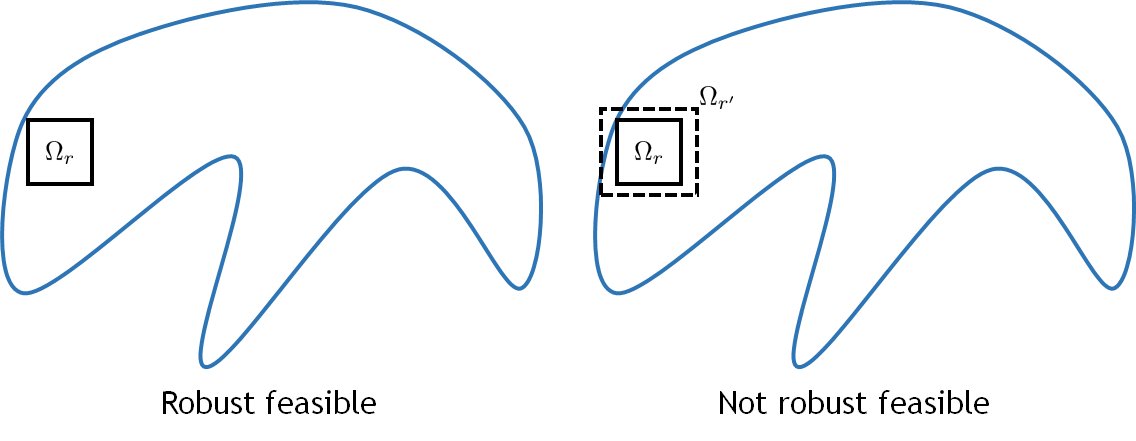
\includegraphics[scale=1.1, bb=0in 0in 5in 2in]{Figures/RobFeas.png} % {Figures/Rfeas}
\end{center}
\caption{Illustration of robust feasibility.
The system is robust feasible at the level of $r$ (left), but is not robust feasible at $r' > r$ (right).}
\label{fig:RFeas}
\end{figure}

The definition for robustness margin is left here in its most general form so as to capture all scenarios under which a researcher may find themselves. 
For instance it very well may be the case that only some of the dimensions of $\vu$ will have margins of uncertainty. 
Furthermore, one may have need of computing the robustness margin for only a subset of the dimensions of $\vu$ which pertain to problem areas or nodes of particular interest to the research. 
This manual restriction will of course produce a robustness margin greater than or equal to that obtained by considering all dimensions, which certainly remains an option under the current setting. 

\section{Theoretical Results} \label{sec:theory}  
We now describe the main technical results of this paper. 
In the first subsection we describe the setting under which the problem can be solved using the results which follow. Our results take advantage of the well studied area of topological degree theory. 
For an introduction to topological degree theory see \cite{OrChCh2006}, \cite{fonseca1995degree} and \cite{MoVrYa2002}. 
Suffice it then to say that should $\Omega\subset\mathbb{R}^{n}$ be open and bounded, $F:\Omega\rightarrow \mathbb{R}$ continuous, and $F(\bold x)\neq \bold y \quad \forall \bold x\in\partial\Omega$ for some $\bold y\in\mathbb{R}^n$, then the degree of $F$ at $y$ over $\Omega$, denoted $d\left(\Omega,F,\bold y\right)\in\mathbb{Z}$, is defined. 
For the purposes of this article we utilize the following property for the degree as our definition of the topological degree of a function $F$ at $y$ over a set $\Omega$. 
See \cite{OrChCh2006} for details.:
\begin{equation}\label{eq:Deg3}
d\left(f,\Omega,\bold y\right)=\sum\limits_{\bold x\in f^{-1}(\bold y)}\operatorname{sign}\left(J_f(\bold x)\right)
\end{equation}

Where $\operatorname{sign}\left(J_f(\bold x)\right)$ denotes the sign of the Jacobian of $F$ at $\bold x$, i.e.:

\[\operatorname{sign}\left(J_f(\bold x)\right)=   \left\{
\begin{array}{ll}
       \ -1   & \mbox{if } J_f(\bold x)< 0, \\
      \quad 0 & \mbox{if } J_f(\bold x)= 0,~\mbox{ and } \\
      \quad 1 & \mbox{if } J_f(\bold x)> 0. \\
\end{array} 
\right. \]

Additionally we utilize the following two common properties of the topological degree. 
See \cite{OrChCh2006} for details. \\
If $H : [0,1]\times\bar{\Omega}\rightarrow\mathbb{R}^n$ is continuous such that $H(t,\bold x)\neq \bold y \quad \forall t\in[0,1]\quad \bold x\in\partial\Omega$,   \ then 
\begin{equation}\label{eq:Deg1} 
d\left(\Omega,H(t,\cdot),\bold y\right)\text{ does not depend on }t.
\end{equation}

\begin{equation}\label{eq:Deg2}
\text{If }d(\Omega,F,\bold y)\neq 0,\text{ then there exists }\bold x\in\Omega\text{ s.t. }F(\bold x)=\bold y. 
\end{equation}


Let $F(\bold x)=Q(\bold x)+L(\bold x)$, $\Omega=\{\bold x| A\bold x< \bold b\}$ and $\hat{\bold x}\in Int(\Omega)$ be a solution to the forecasted system $F(\bold x)=\bold u^*$ in \ref{eq:Quad}, such that $\operatorname{sign}\left(J_{F}(\hat{\bold x})\right)\neq 0$ (for a review of efficient methods of verification see \cite{GRIEWANK2014}). 
If no solutions exist then certainly the system is not robust feasible. Define $\Omega_u=\{\bold u| \bold u\text{ satisfies }\ref{eq:uLimits}\}$.
Verify using existing methods or those adopted from this paper that no other solutions exist in $Int(\Omega)$ (this may require further restricting the domain or even a slight perturbation of the forcasted $\bold u$). 
Thus by \ref{eq:Deg2} and \ref{eq:Deg3} we have verified that $d\left(\Omega, F(\bold x), \bold u^*\right)\neq 0$. 
Note that this is not the only method for verification, but in some sense the easiest to carry out for our purposes. \\

Let $L$ represent an arbitrary line passing through $\bold u^*$, and $\bold l_{min},\bold l_{max}$ the two points of intersection between $\partial\Omega_u$ and $L$. 
Define a homotopy $H_L : [0,1]\times\bar{\Omega}\rightarrow\mathbb{R}^n$ as 
\begin{align}
H_L(t,\bold x) = F(\bold x)-\left[(1-t)\bold l_{min}+t\bold l_{max}\right] \label{eq:Homo}
\end{align}

Observe that by construction $H_L\left(\frac{1}{2},\hat{\bold x}\right)=F(\hat{\bold x})-\bold u^*=\textbf{0}$. 
Thus if no other solutions to $H_L\left(\frac{1}{2},\bold x\right)=0$ exist in $\Omega$ and $\operatorname{sign}\left(J_{H_{L,\frac{1}{2}}}(\hat{\bold x})\right)\neq 0$ then we have that $d(\Omega,H_L\left(\frac{1}{2},\bold x\right),\textbf{0})\neq 0$ by \ref{eq:Deg3}. 
Since $L$ was arbitrary this holds for all such lines passing through $\bold u^*$.\\
Note that for each $\hat{\bold u}\in\Omega_u\setminus\{\bold u^*\}$, $\exists !$ $\hat{L}$ passing through $\bold u^*$ and $t\in[0,1]$,  s.t. $\hat{\bold u}=(1-t)\hat{\bold l}_{min}+t\hat{\bold l}_{max}$. 
Therefore if $d(\Omega,H_L\left(\frac{1}{2},\bold x\right),\bold 0)\neq 0$ for each choice of $L$, it follows by \ref{eq:Deg1} that the robust solvability problem can be determined by validating or invalidating the following statement:
\begin{align}
\not\exists \bold x\in\partial\Omega, \ s.t. \ F(\bold x)-\bold u=\bold 0	 \ \ for \ any \ \ \bold u\in\Omega_u. \label{eq:RSForm}
\end{align}

From here on we will assume $d(\Omega,H\left(\frac{1}{2},\bold x\right),\bold 0)\neq 0$ and focus our efforts on the development of methods for validating or invalidating \ref{eq:RSForm}.\\



\begin{lem} \ \\
\label{lem:BdOpt}
Let $X\subset\mathbb{R}^n$ be closed and $\bold{f}:\mathbb{R}^n\rightarrow\mathbb{R}^n$ be continuous. 
If $\bold{f}$ has no singularities and $$\min\limits_{||\bold{\lambda}||=1}\max\limits_{\bold x\in X}\ \bold{\lambda}^T\bold{f}(\bold x)$$
obtains its optimal at $\bold{\hat{x}}$,$\bold{\lambda}_{\bold{\hat{x}}}$ then $\bold{f}(\bold{\hat{x}})\in \partial \bold{f}(X)$. 
\begin{proof} \ \\
\begin{itemize}
\item[](By contradiction) Assume $\bold{f}(\bold{\hat{x}})\in \bold{f}(X)\setminus\partial \bold{f}(X)$. 
Let $\theta$ the angle between $\bold{\lambda}_{\bold{\hat{x}}}$ and $\bold{\hat{x}}$. 
Thus $\min\limits_{||\bold{\lambda}||=1}\max\limits_{x\in X}\ \bold{\lambda}^T\bold{f}(x)=\bold{\lambda}_{\bold{\hat{x}}}^T\bold{f}(\bold{\hat{x}})=|\bold{f}(\bold{\hat{x}})|\cos(\theta)$. 
Since $X\in\mathbb{R}^n$ is closed it is thus compact which implies $\bold{f}(X)$ is also compact. 
Thus $\exists r>0$ s.t. (ball of radius $r$ centered at $\bold{f}(\bold{\hat{x}})$) $B_r(\bold{f}(\bold{\hat{x}}))\in \bold{f}(X)\setminus\partial \bold{f}(X)$. 
Let $y$ be the antipodal point on $\partial B_r(\bold{f}(\bold{\hat{x}}))$ to the point of intersection between the line segment connecting the origin to $\bold{f}(\bold{\hat{x}})$ and $B_r(\bold{f}(\bold{\hat{x}}))$. 
It follows then that $|y|>|\bold{f}(\bold{\hat{x}})|$ and $\theta$ is the angle between $\bold{\lambda}_x$ and $y$.   
Let $\bold{x^*}\in X$ s.t. $\bold{f}(\bold{x^*})=y$, such a $\bold{x^*}$ exists as $\bold{f}(X)$ is compact. 
Therefore $\bold{\lambda}_{\bold{\hat{x}}}^T\bold{f}(\bold{x^*})=|\bold{f}(\bold{x^*})|\cos(\theta)>|\bold{f}(\bold{\hat{x}})|\cos(\theta)=\bold{\lambda}_{\bold{\hat{x}}}^T|\bold{f}(\bold{\hat{x}})|$ which is a contradiction. 
The lemma now follows.
\end{itemize}
\end{proof}
\end{lem}

\begin{thm} \ \\
\label{thm:MainIneq}
Let $X\subset\mathbb{R}^n$ be closed and $\bold{f}:\mathbb{R}^n\rightarrow\mathbb{R}^n$ be continuous s.t. $\bold{f}(X)$ contains the origin. 
If $\bold{f}$ has no singularities then $$\min\limits_{||\bold{\lambda}||=1}\max\limits_{\bold x\in X}\ \bold{\lambda}^T\bold{f}(\bold x)\geq \min\limits_{\bold x\in \partial X}\max\limits_{||\bold{\lambda}||=1}\ \bold{\lambda}^T\bold{f}(\bold x)$$
\begin{proof} \ \\
\begin{itemize}
\item[] If the origin lies on the boundary of $\bold{f}(X)$ then let $\hat{\bold x}\in \partial X$ s.t. $f(\hat{\bold x})=\textbf{0}$. 
Such an $\hat{\bold x}$ exists as $f$ has no singularities. 
Then  clearly $$\min\limits_{||\bold{\lambda}||=1}\max\limits_{\bold x\in X}\ \bold{\lambda}^T\bold{f}(\bold x)\geq \min\limits_{||\bold{\lambda}||=1}\bold{\lambda}^T\bold{f}(\hat{\bold x})= 0 = \max\limits_{||\bold{\lambda}||=1}\ \bold{\lambda}^T\bold{f}(\hat{\bold x}) \geq \min\limits_{\bold x\in \partial X}\max\limits_{||\bold{\lambda}||=1}\ \bold{\lambda}^T\bold{f}(\bold x)$$
Thus assume the origin lies in the interior of $\bold{f}(X)$.
Let $\bold{\hat{x}}$ be the point and $\bold{\lambda}_{\bold{\hat{x}}}$ the unit vector at which $$\min\limits_{||\bold{\lambda}||=1}\max\limits_{\bold x\in X}\ \bold{\lambda}^T\bold{f}(\bold x)$$
obtains its optimal. \\

Case 1: If the angle, $\theta$, between $\bold{\hat{x}}$ and $\bold{\lambda}_{\bold{\hat{x}}}$ is 0 then $\max\limits_{||\bold{\lambda}||=1}\bold{\lambda}^T\bold{f}(\bold{\hat{x}})=\bold{\lambda}_{\bold{\hat{x}}}^T\bold{f}(\bold{\hat{x}})$. 
Furthermore by \cref{lem:BdOpt} $\bold{f}(\bold{\hat{x}})\in \partial \bold{f}(X)$ and thus $\bold{\hat{x}}\in \partial X$ since $\bold{f}$ has no singularities by hypothesis. 
It follows now that $$\min\limits_{\bold x\in \partial X}\max\limits_{||\bold{\lambda}||=1}\ \bold{\lambda}^T\bold{f}(\bold x)\leq \max\limits_{||\bold{\lambda}||=1}\ \bold{\lambda}^T\bold{f}(\hat{\bold x})=\bold{\lambda}_{\bold{\hat{x}}}^T\bold{f}(\bold{\hat{x}})=\min\limits_{||\bold{\lambda}||=1}\max\limits_{\bold x\in X}\ \bold{\lambda}^T\bold{f}(\bold x)$$

Case 2: Assume $\theta \neq 0$. 
Let $\bold{x^*}$ be a point on the boundary of $X$ s.t. the angle between $\bold{\lambda}_{\bold{\hat{x}}}$ and $\bold{f}(\bold{x^*})$ is 0. 
Such a point must exist as $\bold{f}(X)$ is compact and by hypothesis $\bold{f}(X)$ contains the origin, has no singularities ($\bold{f}$ maps $\partial X$ to $\partial \bold{f}(X)$) and by assumption the origin lies in the interior of $\bold{f}(X)$. 
It follows then that $$\min\limits_{\bold x\in \partial X}\max\limits_{||\bold{\lambda}||=1}\ \bold{\lambda}^T\bold{f}(\bold x)\leq \max\limits_{||\bold{\lambda}||=1}\bold{\lambda}^T \bold{f}(\bold{x^*}) =\bold{\lambda}_{\bold{\hat{x}}}^T\bold{f}(\bold{x^*})\leq \max\limits_{\bold x\in X}\bold{\lambda}_{\bold{\hat{x}}}^T\bold{f}(\bold x)=\min\limits_{||\bold{\lambda}||=1}\max\limits_{\bold x\in X}\ \bold{\lambda}^T\bold{f}(\bold x)$$

The theorem now follows.
\end{itemize}
\end{proof}
\end{thm}

\cref{thm:MainIneq} and \cref{lem:BdOpt} provide us with the theoretical tools we need to develop models for approximating the robustness margin.
We will use the terminology "inner bound models" to describe the process of verifying robust feasibility while expanding the uncertainty box centered at $\bold u^*$ in order to compute the lower bounds on the robustness margin, which these models undertake. 
We use the terminology "outer bound models" to capture in a similar fashion the procedure used to compute the upper bounds on the robustness margin by contracting the uncertainty box until the system may be robust feasible. 
As such we dedicate the remainder of this section to the development of these inner and outer bound formulations. 

\section{Inner Bound Models} \label{sec:inbdform}  
\section{Computing Lower Bounds on the Robustness Margin} \label{sec:inbdform}

In this section we will derive procedures for computing a lower bound on the robustness margin. 
We start with an exact formulation, which turns out to be hard to implement efficiently in practice.
Hence we relax the procedures until they become computationally tractable. 
We end the section by providing three different implementations of our final derived, relaxed, computationally tractable procedure specified in Equation (\ref{eq:OPTfeasrelax}).
Each of these three practical implementations brings a unique set of attributes, which makes none of them the clearly preferred candidate.

\smallskip
\begin{thm}
  Let $\Omega=\{\vx| A\vx \leq \vb\}$, $\Omega_{u}=\{\vu| u^{\min}_i\leq u_i \leq u^{\max}_i \ \forall i \}$, and $F(\vx)=Q(\vx)+L\vx$ as described in Equations (\ref{eq:Quad}), (\ref{eq:xLimits}), and (\ref{eq:uLimits}). 
  Let
  \[
  z = \min\limits_{\vx\in \partial \Omega, \vu\in \Omega_{u} }\max\limits_{\norm{\vlambda}=1}\ \vlambda^T\left(F(\vx)-\vu\right).
  \]
  If there is an $r>0$ such that $r \leq e_i \ \forall i$ with $\ e_i>0$, where $e_i$ denotes the error bounds associated with $ u^{\min}_i$ and $ u^{\max}_i$, and if $z > 0$ then the system is robust feasible and has a robustness margin of at least $r$.

  \medskip
  \begin{proof} 
    If \cref{eq:RSForm} is invalidated then there exists $\hat{\vx} \in \partial\Omega$ such that. $F(\hat{\vx})=\hat{\vu}$ for some $\hat{\vu}\in\Omega_{u}$ and thus
    \[
    z = \min\limits_{\vx\in \partial \Omega}\max\limits_{\norm{\vlambda}=1}\ \vlambda^T\left(F(\vx)-\vu\right) ~\leq~ \max\limits_{\norm{\vlambda}=1, \vx=\hat{\vx}}\ \vlambda^T\left(F(\vx)-\hat{\vu}\right) ~=~ 0.
    \]
    Hence if $z>0$, \cref{eq:RSForm} is validated, and the system is robust feasible.
    It follows then by definition that the system has a robustness margin of at least $r$.
  \end{proof}
\end{thm}

  \medskip
\begin{thm} \label{thm:RobFeas}
  Let $\partial\Omega_i=\{\vx| (A\vx)_i = b_i, A\vx\leq \vb\}$, $\Omega_{u}=\{\vu| u^{\min}_i\leq u_i \leq u^{\max}_i \ \forall i \}$, and $F(\vx)=Q(\vx)+L(\vx)$ as described in \cref{eq:Quad,eq:xLimits,eq:uLimits}.
  Define
  \begin{align}
    \rz_i =  \min_{\vx\in\partial\Omega_i, \vu \in \Omega_u} \norm{F(\vx)-\vu}. \label{eq:OPTfeas}
  \end{align}
  The system is robust feasible if and only if $\rz_i>0$ for each $i = 1, \ldots, m$, where $m$ is the number of rows of $A$.
%If $\rz_i>0$ for each $i = 1, \ldots, m$ (where $m$ is the number of rows of $A$), then the system is robust feasible.

  \begin{proof} \ \\
    $\boxed{\Rightarrow}$ \\ 
    If the system is not robust feasible then there exists $\hat{\vu}'\in \Omega_u$ such that $F(\vx)=\hat{\vu}'$ has no solution. 
    Since $F(\vx)=\vu^*$ has a solution and $F$ is continuous over a compact domain, there must exist an $\hat{\vx} \in \Omega = \{\vx| A\vx \leq \vb\}$ such that $F(\hat{\vx})=\hat{\vu}$ for some $\hat{\vu}\in \Omega_u\cap \partial F(X)$. 
    Since $\partial F(X) = F(\partial X)$ we have that $\hat{\vx}\in\partial\Omega$, which implies that there is an $i$ such that $A\hat{\vx}_i=b_i$, and thus $0 \leq \rz_i \leq \norm{F(\hat{\vx})-\hat{\vu}}=0$.\\
    %
    $\boxed{\Leftarrow}$ \\ 
    If there exists an $i$ such that $\rz_i = 0$, then there must exist an $\hat{\vx} \in \partial\Omega $ and $\hat{\vu}\in \Omega_u$ such that $F(\hat{\vx})=\hat{\vu}$. 
    Since $\partial F(X) = F(\partial X)$, there cannot exist an $\hat{\vx}' \in \Int\Omega$ such that $F(\hat{\vx}')=\hat{\vu}$, and hence by definition the system is not robust feasible.
    %\cref{eq:RSForm} is invalidated, which implies $\exists \hat{\vx}\in\partial\Omega$, $\Omega=\{\vx| A\vx< \vb\}$, such that $F(\hat{\vx})=\hat{\vu}$ for some $\hat{\vu}\in \Omega_u$. 
    %Since $\hat{\vx}\in\partial\Omega$ this implies that $\exists i$ such that $A\hat{\vx}_i=b_i$ and thus $0\leq \rz_i \leq ||F(\hat{\vx})-\hat{\vu}||=0$.
    %Thus if $\rz_i>0$ for each $i = 1, \ldots, m$, \cref{eq:RSForm} is validated, and the system is robust feasible.
  \end{proof}
\end{thm}

%Note that under these circumstances $\min\limits_{\norm{\vlambda}=1}\max\limits_{x\in \bar{\Omega}}\ \vlambda^T\left(F(x)-\hat{u}\right)> 0$ is possible, especially if $F(\bar{\Omega})$ is highly non-convex. However, should $\exists u^{\prime}$ such that $\min\limits_{\norm{\vlambda}=1}\max\limits_{x\in \bar{\Omega}}\ \vlambda^T\left(F(x)-u^{\prime}\right)=0$ then by \ref{MainInEqLem} we know that there $\exists \hat{x}\in\partial\Omega$ such that $F(\hat{x})=u^{\prime}$. Hence the following formulation of an outer bound approximation on $u_i^{\min}$ and $u_i^{\max}$:


The optimization problems presented in \cref{thm:RobFeas} are nonlinear and nonconvex.
Hence it may be difficult to solve them in general.
In fact, since $F(\vx)$ is quadratic in $\vx$, they are quadratically constrained quadratic programs (QCQPs), which are NP-hard in general \cite{PaBo2017}.
At the same time, we can use well known \emph{semidefinite programming relaxations for QCQPs} to obtain lower bounds on the optimal values \cite{VaBo1996}.
Since $Q$ is quadratic, it can also be written as a linear function of $\vx\vx^T$.
More concretely, we can write
$$Q(\vx)_i=\vx^TQ_i\vx=\Tr(Q_i\vx\vx^T)$$
where each $Q_i$ is as defined in \cref{eq:Quad}. 
Since $\vx$ should satisfy $A\vx\leq \vb$, we get
\[
  (\vb-A\vx)(\vb-A\vx)^T \geq 0~~\Rightarrow~~ \vb\vb^T-A\vx\vb^T-\vb(A\vx)^T+A(\vx\vx^T)A^T\geq 0.
\]
If we allow a symmetric positive semidefinite matrix $X$ to take the place of $\vx\vx^T$ and drop the rank constraint ($\rank(X)=1$)) we can construct the following relaxation for the optimization problem presented in \cref{thm:RobFeas}:
% 
\begin{equation}\label{eq:OPTfeasrelax}
  \begin{array}{rl}
    \hat{\rz}_{i} = & \min\limits_{\vx}  b_i-(A\vx)_i  \\
    \vspace*{-0.05in} \\
%\begin{align*}
    \text{subject to } \ & \Tr\left(Q_iX\right)+ L_i\vx \geq \vu_i^{\min} \ \ \forall i\\
    & \Tr\left(Q_iX\right)+ L_i\vx \leq \vu_i^{\max} \ \ \forall i\\
    &A\vx\leq \vb \\
    &\vb\vb^T-A\vx\vb^T-\vb(A\vx)^T+AXA^T\geq O \\
    &X \text{ is symmetric and positive semidefinite.}
  \end{array}
\end{equation}
%\end{align*}
%
Here $L_i$ denotes the $i^{\rm th}$ rows of $L$, and $O$ denotes the $2n \times 2n$ matrix of zeros with the constraints understood to be component-wise inequalities.
Note that if we impose $\rank(X)=1$, we do get an exact formulation.
At the same time, it may be difficult to impose this constraint.
But the system (in \cref{eq:OPTfeasrelax}) without the rank constraint is a convex optimization problem (a semidefinite program, in fact) and can be solved efficiently. 
Since this is a relaxation of the procedure described in \cref{thm:RobFeas}, if $\hat{\rz}_i>0$ for each $i$, the condition in \cref{thm:RobFeas} (i.e., $\rz_i>0 \ \forall i$) is satisfied. 
We can further relax the formulation in \cref{eq:OPTfeasrelax} by dropping the condition that $X$ be positive semidefinite, which transforms the problem from a semidefinite program to a linear program. 
We now present three formulations for this new, relaxed program, and provide numerical results for each of them in \cref{ssec:compres}.
We also describe the advantages and drawbacks of each formulation.

\bigskip
\bigskip
\textbf{LP Feasibility Procedure} 
\begin{equation} \label{eq:OPTfeasrelaxLP1}
\begin{array}{rl}
 &\text{Find an }\vx \\
 \text{subject to } \ &(A\vx)_i= b_i \\
 &\Tr\left(Q_iX\right)+ L_i\vx \geq \vu_i^{\min}  \ \ \forall i\\
 & \Tr\left(Q_iX\right)+ L_i\vx \leq \vu_i^{\max}  \ \ \forall i\\
 	&A\vx\leq \vb \\
 	&\vb\vb^T-A\vx\vb^T-\vb(A\vx)^T+AXA^T\geq O \\
 	&X \text{ is symmetric.}
\end{array}
\end{equation}


This procedure has the advantage of being a linear program and hence can be solved efficiently.
But as noted by the objective $\rz_i$, one must iterate over each dimension of $A\vx$ checking feasibility of the procedure. 
Of course, should the procedure prove feasible then we have found a solution on the boundary and thus invalidating the Statement in (\cref{eq:RSForm}). 
If the procedure proves infeasible then we are free to push the robustness margin higher and test again. 
An alternative approach is to consider all of the dimensions of $A\vx$ simultaneously by introducing extra binary variables and creating a MIP as follows. 

\bigskip
\textbf{MIP Procedure}\
\begin{equation}\label{eq:OPTfeasrelaxLP2}
\begin{array}{rl}
\max &  z  \\
 \text{subject to } \ &\Tr\left(Q_iX\right)+ L_i\vx \geq \vu_i^{\min}  \ \ \forall i\\
 & \Tr\left(Q_iX\right)+ L_i\vx \leq \vu_i^{\max}  \ \ \forall i\\
 	&A\vx\leq \vb \\
 	&\vb\vb^T-A\vx\vb^T-\vb(A\vx)^T+AXA^T\geq O \\
 	&X \text{ is symmetric} \\
 	& z\leq (A\vx)_i-b_i+R(1-d_i) \ \forall i \ \text{ for some large enough $R$} \\
 	& \sum\limits_i d_i=1 \\
 	& d_i\in\{0,1\} \ \forall i .
\end{array}
\end{equation}


The MIP and LP Feasibility procedures are similar and should theoretically give the same results. 
However, as we will show in our numerical studies, the LP Feasibility procedure could outperform the MIP procedure by producing higher robustness margins and running faster in higher dimensions. 
In both procedures, the process ends after a boundary solution is found. 
This solution may not be a boundary solution to the actual system, but may be an artifact of the relaxations used to create the procedures. 
One way of tackling this issue is by updating the constraints using an iterative process as outlined in the following procedure.

\bigskip
\textbf{LP Bound Tightening Procedure}
\begin{equation}\label{eq:OPTfeasrelaxLP3}
\begin{array}{rl}
\max &  z_i = (A\vx)_i  \\
 \text{subject to } \ &\Tr\left(Q_iX\right)+ L_i\vx \geq \vu_i^{\min}  \ \ \forall i\\
 & \Tr\left(Q_iX\right)+ L_i\vx \leq \vu_i^{\max}  \ \ \forall i\\
 	&A\vx\leq \vb \\
 	&\vb\vb^T-A\vx\vb^T-\vb(A\vx)^T+AXA^T\geq O \\
 	&X \text{ is symmetric.}
\end{array}
\end{equation}

What distinguishes the LP Bound Tightening procedure from the other two procedures is the ability to use it iteratively by updating the constraints of \cref{eq:OPTfeasrelaxLP3}, replacing $\vb$ with $\vz$, the vector of $z_i$'s found after running the procedure over all dimensions of $A\vx$. 
Since clearly $\vz \leq \vb$, we have that the polytope $\{\vx ~|~ A\vx\leq \vz\} \, \subseteq \, \{\vx ~|~ A\vx\leq \vb\}$. 
Thus it follows that any system deemed robust feasible using \cref{eq:OPTfeasrelaxLP1} or \cref{eq:OPTfeasrelaxLP2} will certainly be found robust feasible using \cref{eq:OPTfeasrelaxLP3}, but a system found robust feasible using \cref{eq:OPTfeasrelaxLP3} may not be found robust feasible using \cref{eq:OPTfeasrelaxLP1} or \cref{eq:OPTfeasrelaxLP2}. 
The drawback of the bound tightening procedure, as we shall see in the Computational Results (\cref{ssec:compres}), is choice of parameters to be manually set in order to tell the procedure when to stop. 


\section{Outer Bound Models} \label{sec:outbdform}  
\section{Computing Upper Bounds on the Robustness Margin} \label{sec:outbdform}  

As a result of the complexity of $\displaystyle \min\limits_{\vx\in \partial \Omega, \vu\in\Omega_u}\max\limits_{||\boldsymbol{\lambda}||=1 }\ \boldsymbol{\lambda}^T\left(F(\vx)-\vu\right)$ we derived a sequence of relaxations in order to arrive at a method that was computationally efficient for a non-trivial data set. 
We can similarly work with $\displaystyle \min\limits_{||\boldsymbol{\lambda}||=1}\max\limits_{\vx\in \bar{\Omega}, \vu\in\Omega_u}\ \boldsymbol{\lambda}^T\left(F(\vx)-\vu\right)$ to produce computationally efficient models for outer bound approximations of the robustness margin. 
\begin{thm}\label{thm:OPTfeasOut} 
Let $\bar{\Omega}=\{\vx| A\vx\leq \vb\}$, $\Omega_{u}=\{\vu| u^{\min}_i\leq u_i \leq u^{\max}_i \ \forall i \}$, and $F(\vx)=Q(\vx)+L(\vx)$ as described in \cref{eq:Quad}, \cref{eq:xLimits} and \cref{eq:uLimits}. 
Let
$$z = \min\limits_{||\boldsymbol{\lambda}||=1}\max\limits_{\vx\in \bar{\Omega}, \vu\in\Omega_u}\ \boldsymbol{\lambda}^T\left(F(\vx)-\vu\right).$$
If $r>0$ such that $r\leq e_i \ \forall i \ such that \ e_i>0$ where $e$ denotes the error bounds associated with $ u^{\min}_i$ and $ u^{\max}_i$, and if $z=0$ then the system has robustness margin of no more than r.

\begin{proof} 
  Observe by \cref{lem:BdOpt} that if $\min\limits_{||\boldsymbol{\lambda}||=1}\max\limits_{\vx\in \Omega, \vu\in\Omega_u}\ \boldsymbol{\lambda}^T\left(F(\vx)-\vu\right)=0$, then \cref{eq:RSForm} is invalidated.  

%Observe that if \cref{eq:RSForm} is invalidated then $\exists \hat{x}\in\partial\Omega$ such that $F(\hat{x})=\hat{u}$ for some $\hat{u}\in\Omega_{u}$ and thus certainly $$\min\limits_{||\boldsymbol{\lambda}||=1}\max\limits_{x\in X, u\in\Omega_u}\ \boldsymbol{\lambda}^T\left(F(x)-u\right) \geq \min\limits_{||\boldsymbol{\lambda}||=1}\ \boldsymbol{\lambda}^T\left(F(\hat{x})-\hat{u}\right)=0.$$ The theorem now follows.
%\end{itemize}
\end{proof}
\end{thm}

We can relax the model in \cref{thm:OPTfeasOut} utilizing the same techniques as before, replacing $\vx\vx^T$ with a positive semidefinite matrix $X$, with the option of dropping the condition that $X$ be positive semidefinite, which transforms the model from a semidefinite program to a linear or mixed integer program depending on how one deals with the condition $||\boldsymbol{\lambda}||=1$. 
In our tests we iterate over all possible sign choices for each dimension of $\boldsymbol{\lambda}$ as there are only ten dimensions of variability in our applications. \\

\textbf{Outer Bound Model A}
\begin{equation}\label{eq:OPTfeasOutRelaxa}
\begin{array}{rl}
 \ z &=\min\limits_{||\boldsymbol{\lambda}||=1}\max\limits_{\vx} \boldsymbol{\lambda}^T\left(F(\vx)-\vu^*\right) \\
 \text{subject to: } \ & A\vx\leq \vb \\
 	&\vb\vb^T-A\vx\vb^T-\vb(A\vx)^T+A\mathcal{X}A^T\geq O \\
 	&\mathcal{X} \text{ is symmtric}
\end{array}
\end{equation}


We can construct the dual of the inner maximal objective of \cref{eq:OPTfeasOutRelaxa} to produce: \\

\textbf{Outer Bound Model B} 
\begin{equation}\label{eq:OPTfeasOutRelaxb}
\begin{array}{rl}
\ z &=\min\limits_{||\boldsymbol{\lambda}||=1,\vy}B^T\vy  \\
 \text{subject to: } \ & H^T\vy=\vu(\lambda) \\
 & \vy\leq 0
\end{array}
\end{equation}
where the constraints of \cref{eq:OPTfeasOutRelaxa} can be written as $H\vx\geq B$ and the objective of \cref{eq:OPTfeasOutRelaxa} as $\vu(\lambda)^T\vx$. 
Notice that the objective of \cref{eq:OPTfeasOutRelaxa} is different from that of \cref{thm:OPTfeasOut}. 
The optimal value of the objectives of  \cref{eq:OPTfeasOutRelaxa} and \cref{eq:OPTfeasOutRelaxb} are much easier to find and they allow us to directly solve for the minimal outer bound approximation of the robustness margin. 


\section{Numerical Studies} \label{sec:numstd}  
\section{Numerical Studies} \label{sec:numstd}  

Robust feasibility of systems of nonlinear equations has been studied in a series of recent papers \cite{FrKr2015,FrKrWa2016}.
These studies show that the problem is decidable (a terminating algorithm guaranteed to produce an answer exists) as long as the number of variables is not more than twice the number of equations minus $3$.
In our main application domain, we are primarily concerned with the AC power flow equations
%\eqref{eq:ACPF},
where the number of equations is the same as the number of variables, and hence the aforementioned algorithm \cite{FrKr2015,FrKrWa2016} applies to problem \ref{RobustDef}.
However, the algorithm requires computing a simplicial decomposition of the domain set (a triangulation).
The algorithm scales as $\tilde{O}(s^4)$ where $s$ is the number of simplices in the complex.
Further, the number of simplices in a simplicial decomposition grows exponentially with the dimension $n$, severely limiting the scalability of these algorithms to realistically-sized power grids ($n=1000$ or higher).

Specific to power systems, there has been significant empirical work on solving the PF equations with probabilistic uncertainty \cite{morales2007point,wang1992interval}.
However, these algorithms are based on sampling heuristics and do not offer mathematical guarantees of robust feasibility.
There has been recent work on specifying conditions on the power injections over which the power flow equations are guaranteed to have a solution \cite{bolognani2016existence,EPFLA,EPFLB}.
However, they do not directly address the robust feasibility problem, and using these regions to assess robust feasibility can produce very conservative results.
Further, they do not address uncertainty in the quadratic and linear objective terms.

We now present computational studies which support the efficiency of the models we have presented, which address the aforementioned short comings of previous work. 
For all the numerical results presented we apply models \eqref{eq:OPTfeasOutRelaxb}, \eqref{eq:OPTfeasrelaxLP1}, \eqref{eq:OPTfeasrelaxLP2}, and \eqref{eq:OPTfeasrelaxLP3} to find upper and lower bounds for the robustness margins with respect to the optimal power flow equations derived using datasets obtained from the MatPower package found in the MATLAB software, see \cite{matpower}. 
We will specifically show results for tests conducted on cases 5, 9, 14, 30 and 57. 
In every case the power flow equations were converted into the format defined by \eqref{eq:Quad}, \eqref{eq:xLimits}, and \eqref{eq:uLimits}. 
To simulate real life scenarios we allowed the first 5 dimensions of $\bold u$ to represent renewable energy, and the others representing no variation. We then slowly increased the variation of the first 5 dimensions of $\bold u$, while utilizing models \eqref{eq:OPTfeasOutRelaxb} for the outer bound, and \eqref{eq:OPTfeasrelaxLP1}, \eqref{eq:OPTfeasrelaxLP2} and \eqref{eq:OPTfeasrelaxLP3} for the inner bound verification to verify robust feasibility. 
The following subsection will detail specifically how this transformation was conducted.
\subsection{OPF to Quadratic System}
As described in \cite{DjTuritsyn}, the AC power flow equations can be written as 
\begin{align}\label{eq:Real1}
& Re\left(\sum\limits_{k=1}^n V_i\left(\overline{Y_{ik}V_k} + \overline{Y_{i0}V_0}\right)\right) = p_i \ \forall i\in PQ \\
& Im\left(\sum\limits_{k=1}^n V_i\left(\overline{Y_{ik}V_k} + \overline{Y_{i0}V_0}\right)\right) = q_i \ \forall i\in PQ \\
& Re\left(\sum\limits_{k=1}^n V_i\left(\overline{Y_{ik}V_k} + \overline{Y_{i0}V_0}\right)\right) = p_i \ \forall i\in PV \\
& |V_i|^2 = v_i, \  \ \forall i \in PV 
\end{align}

where $V_i$ denotes the complex voltage phasor, $p_i$ the active and $q_i$ the reactive power injection, and $Y$ the admittance matrix at node $i$. $PV$ denotes the set of $PV$ nodes, $PQ$ denotes the set of $PQ$ buses and $v_i$ denotes the squared voltage magnitude setpoints at the $PV$ buses. We can then rewrite \ref{eq:Real1} into the system outlined by \ref{eq:Quad}, \ref{eq:xLimits}, and \ref{eq:uLimits} with 
$x=\left(Re(V_1), \dots, Re(V_n), Im(V_1),\dots , Im(V_n)\right)$ and $u=\left(p_1, \dots, p_n, q_1, \dots, q_n, v_1, \dots, v_n\right)$. 


\subsection{Computational Results}


The modeling was conducted with $A\bold x\leq \bold b = B*ones$ for $B\in\{0.001, 0.005,0.01\}$ and $ones$ representing the vector of all ones of appropriate dimension. 
$A$ in this cases is a matrix s.t. $A\bold x\leq \bold b$ controls the flow between nodes in the power grid (i.e. each row of $A\bold x\leq \bold b$ has the form $x_i-x_j\leq b_k$. 
All computations were performed on a laptop running the 64bit Windows 10 operating system containing an Intel i-7 processor, 16 GB of Ram and 4 cores. 
Graphically we can look at this data on a case by case basis to highlight the effect of allowing more fluctuation between the nodes (i.e. as $B$ increases).(Figure \ref{fig:Graphs1}) 

%\begin{figure}[h]
%\begin{center}
%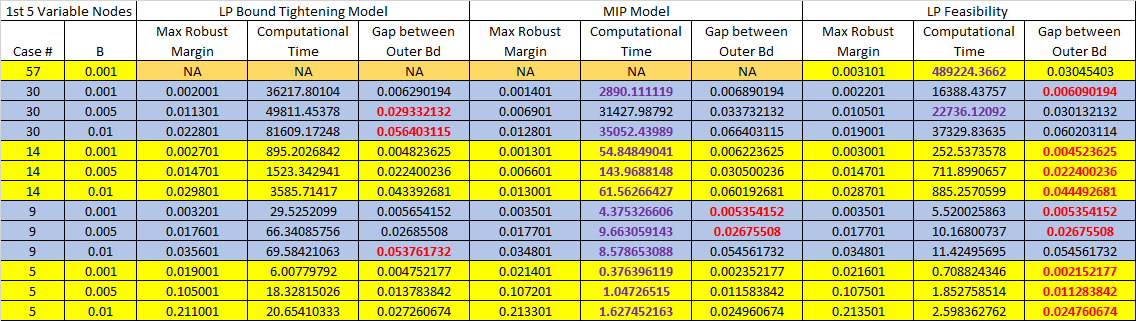
\includegraphics[scale=0.4]{Figures/InnerBoundTable} 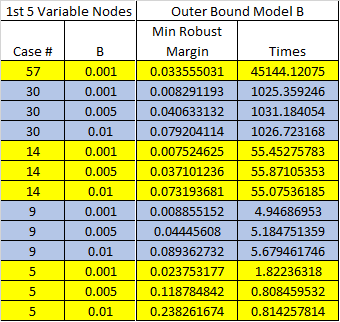
\includegraphics[scale=0.4]{Figures/OuterBoundTable} 
%\end{center}
%\label{tbl:Table1}
%\end{figure} 

\begin{figure}[htp!]
\begin{center}
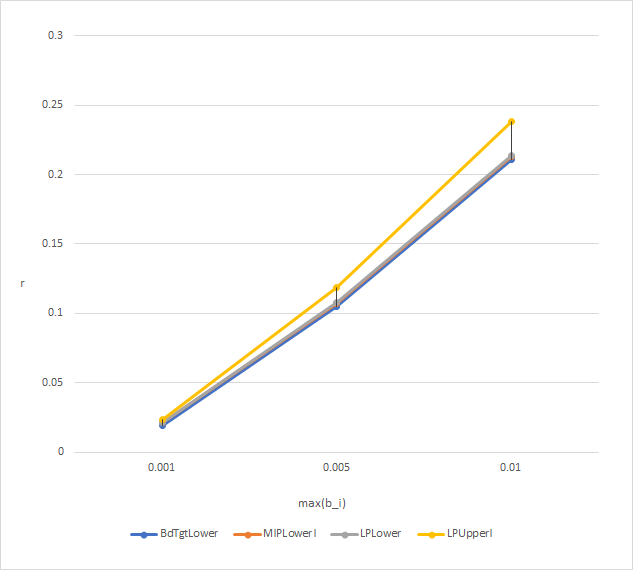
\includegraphics[scale=0.45]{Figures/Case5}
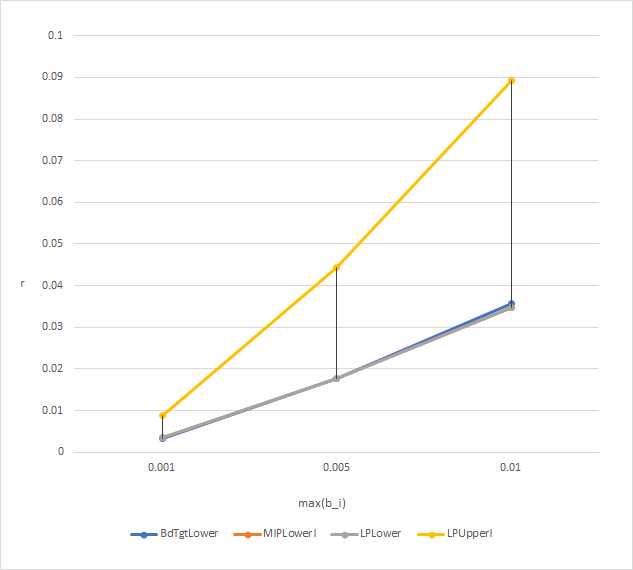
\includegraphics[scale=0.45]{Figures/Case9} \\
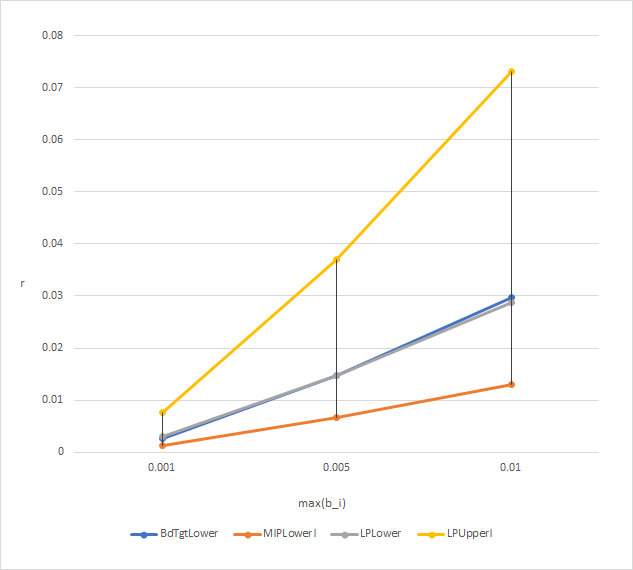
\includegraphics[scale=0.45]{Figures/Case14}
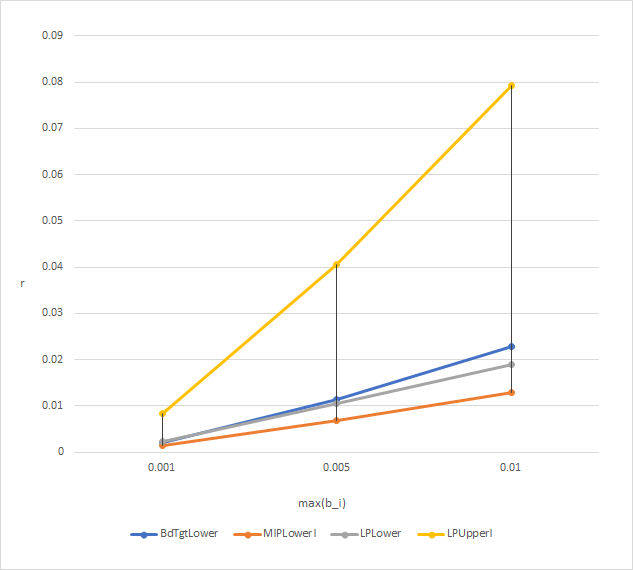
\includegraphics[scale=0.45]{Figures/Case30}
\caption{Case 5 (Top Left), Case 9 (Top Right), Case 14 (Bottom Left), Case 30 (Bottom Right)} 
\label{fig:Graphs1} 
\end{center}
\end{figure}

Case 57 is not included in the graphs as the only inner bound model to run in any reasonable time was the Feasibility model that produced a max robust margin of $\approx$0.003 with a computational time of $\approx$489224 and a gap to the outer bound model, which had a running time $\approx$45144, of $\approx 0.030$ when $B=0.001$.
As evident from the graphs we have that the bound tightening model produces a better approximation of the inner bound on the robustness margin as the complexity of the data set increases. 
Certainly one would expect the bound tightening model to out perform the other inner bound models for all cases, but the choice of model parameters has a big effect on the efficiency of the model. 
For instance, setting a low tolerance for a minimal sufficient change in the dimensions of $\bold b$ will cause in most cases an extremely long running time. 
Thus in the extremely low and marginally high complexity cases it should be expected that the other models will out perform the bound tightening model as these manually set model parameters will have more of an impact on performance. 
Of special interest is the difference in performance of the MIP and Feasibility inner bound models as the complexity of the data increases. 







\section{Discussion} \label{sec:disc}

\delete{Need to add mode details...}

We have proposed novel and efficient techniques for determining robust solvability of quadratic systems with uncertainty. 
It is worth mentioning that the same machinery can be used to determine robustness margins of solutions to static systems by taking $A$ to be the identity, $e_i=0 \ \forall i$ and simply adjusting $\vb$ accordingly. 
The models presented here are in some sense just the tip of the iceberg. 
More efficient models can certainly be derived using the theory contained here. 
We present these models only as examples of how efficient algorithms could be constructed utilizing the theoretical results we presented. 


\section*{Acknowledgment}

Krishnamoorthy, Luo, and Rapone acknowledge funding from the National Science Foundation through grants 1661348 and 1819229.
Dvijotham and Rapone were supported by the Pacific Northwest National Laboratory (PNNL) Center for Complex Systems Initiative while working on this project. 


\bibliographystyle{plain}
\bibliography{Ref}

\end{document}
